% Settings for the default beamer theme
\documentclass[english, aspectratio=169]{beamer}
\usepackage[T1]{fontenc}
\usepackage[utf8]{inputenc}
\usepackage{tabularx}
\usepackage{babel}
\usepackage[ruled,vlined]{algorithm2e}
\SetAlgorithmName{Algoritmus}{algoritmus}{List of Algorithms}
\setcounter{secnumdepth}{3}
\setcounter{tocdepth}{3}

\makeatletter

\newcommand\makebeamertitle{\frame{\maketitle}}

% (ERT) argument for the TOC
\AtBeginDocument{%
  \let\origtableofcontents=\tableofcontents
  \def\tableofcontents{\@ifnextchar[{\origtableofcontents}{\gobbletableofcontents}}
  \def\gobbletableofcontents#1{\origtableofcontents}
}

% Theme settings
\usetheme{Frankfurt}
\usecolortheme{default}
\usefonttheme[onlymath]{serif}

% Template settings
\setbeamertemplate{navigation symbols}{}
\setbeamertemplate{blocks}[rounded][shadow=false]
\setbeamertemplate{title page}[default][colsep=-4bp, rounded=true, shadow=false]
\makeatother

\begin{document}

% Title page
\section{Bevezetés}
\title[]{Üzleti Intelligencia}
\subtitle{7. Előadás: Mesterséges mélytanulás}
\author[Kuknyó Dániel]{Kuknyó Dániel\\Budapesti Gazdasági Egyetem}
\date{2023/24\\1.félév}
\makebeamertitle

% Table of contents slide
\begin{frame}
\tableofcontents{}
\end{frame}

% Table of contents of the current section
\begin{frame}
\tableofcontents[currentsection]
\end{frame}

\begin{frame}{Biológiai és mesterséges neuronok}
\begin{columns}
\begin{column}{.5\textwidth}
Az ember találmányait mindig a természet ihlette. A repülőgépeket a madarak mintájára, a gépkocsit a lovak inspirálták. A természetes lépés ezután az volt, hogy az emberi agyat is modellezik.\par\medskip
Az első perceptron modellt Warren McCulloh és Walter Pitts hozta létre, először pedig Frank Rosenblatt épített egy perceptron gépet. Ez egy képfelismerő gép volt, 400 véletlenszerűen kapcsolt fotocella volt az érzékelője. A súlyokat potenciométerek implementálták, és a súlyok frissítését elektromotorok hajtották végre. 
\end{column}
\begin{column}{.5\textwidth}
\begin{center}
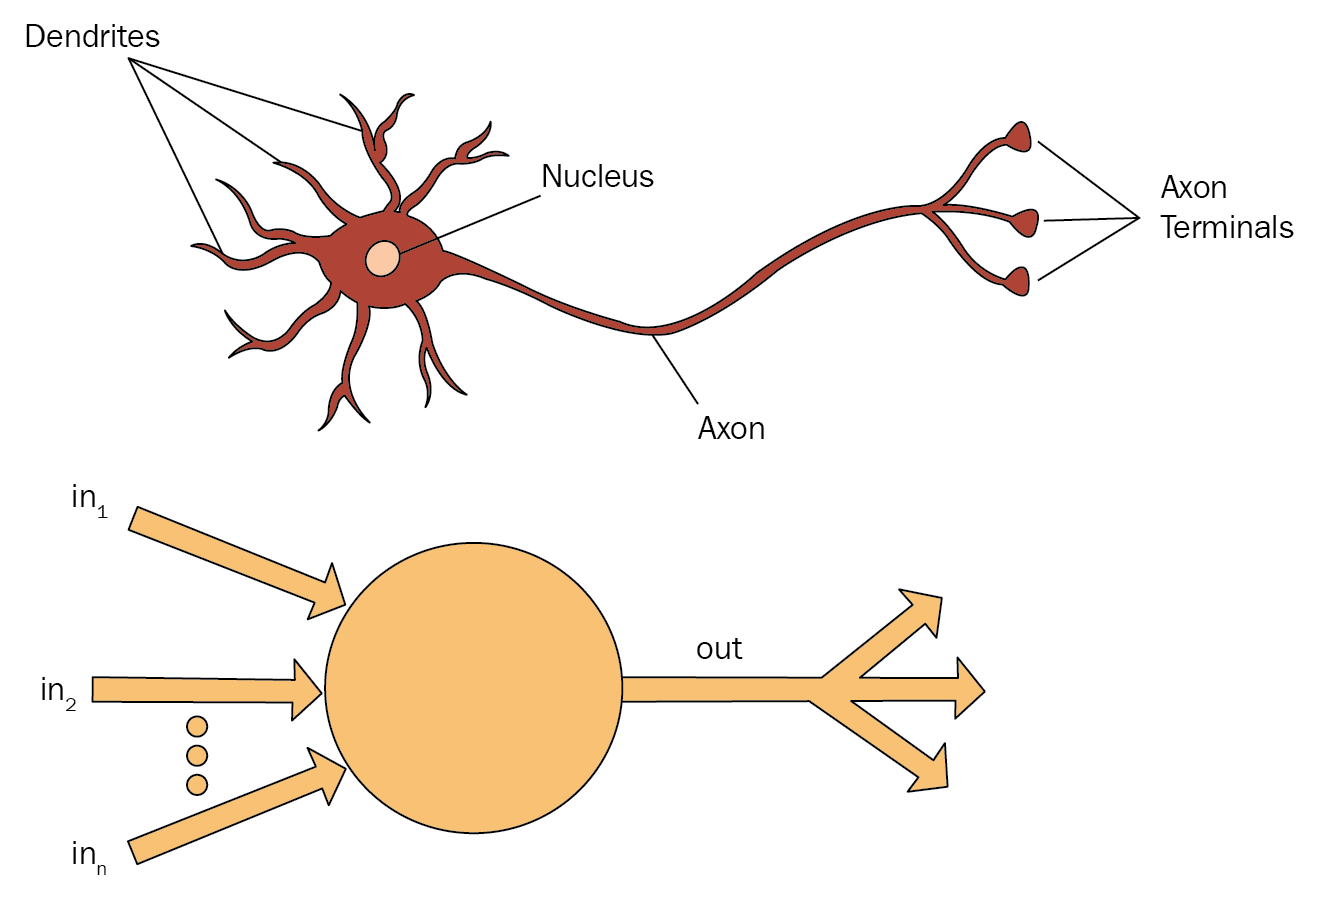
\includegraphics[width=7cm, keepaspectratio]{images/dl_1.png}
\end{center}
\end{column}
\end{columns}
\end{frame}

\begin{frame}{A neuron}
\begin{columns}
\begin{column}{.4\textwidth}
Az egyes neuronok egyszerű elemi műveleteket végeznek. A neuronnak több $x$ inputja (kapcsolata) van, és mindegyikhez egy $w$ \textbf{súly} tartozik.\par\smallskip
A neuron kiszámítja az inputjainak a súlyozott összegét 
\begin{block}{}
\vspace{-0.5cm}
\[
z=x_1w_1 + x_2w_2 + ... + x_nw_n
\]
\end{block}
majd ezt az értéket behelyettesíti egy aktivációs függvénybe:
\begin{block}{}
\vspace{-0.1cm}
\[
h=\varphi(z)
\]
\end{block}
\end{column}
\begin{column}{.6\textwidth}
\begin{center}
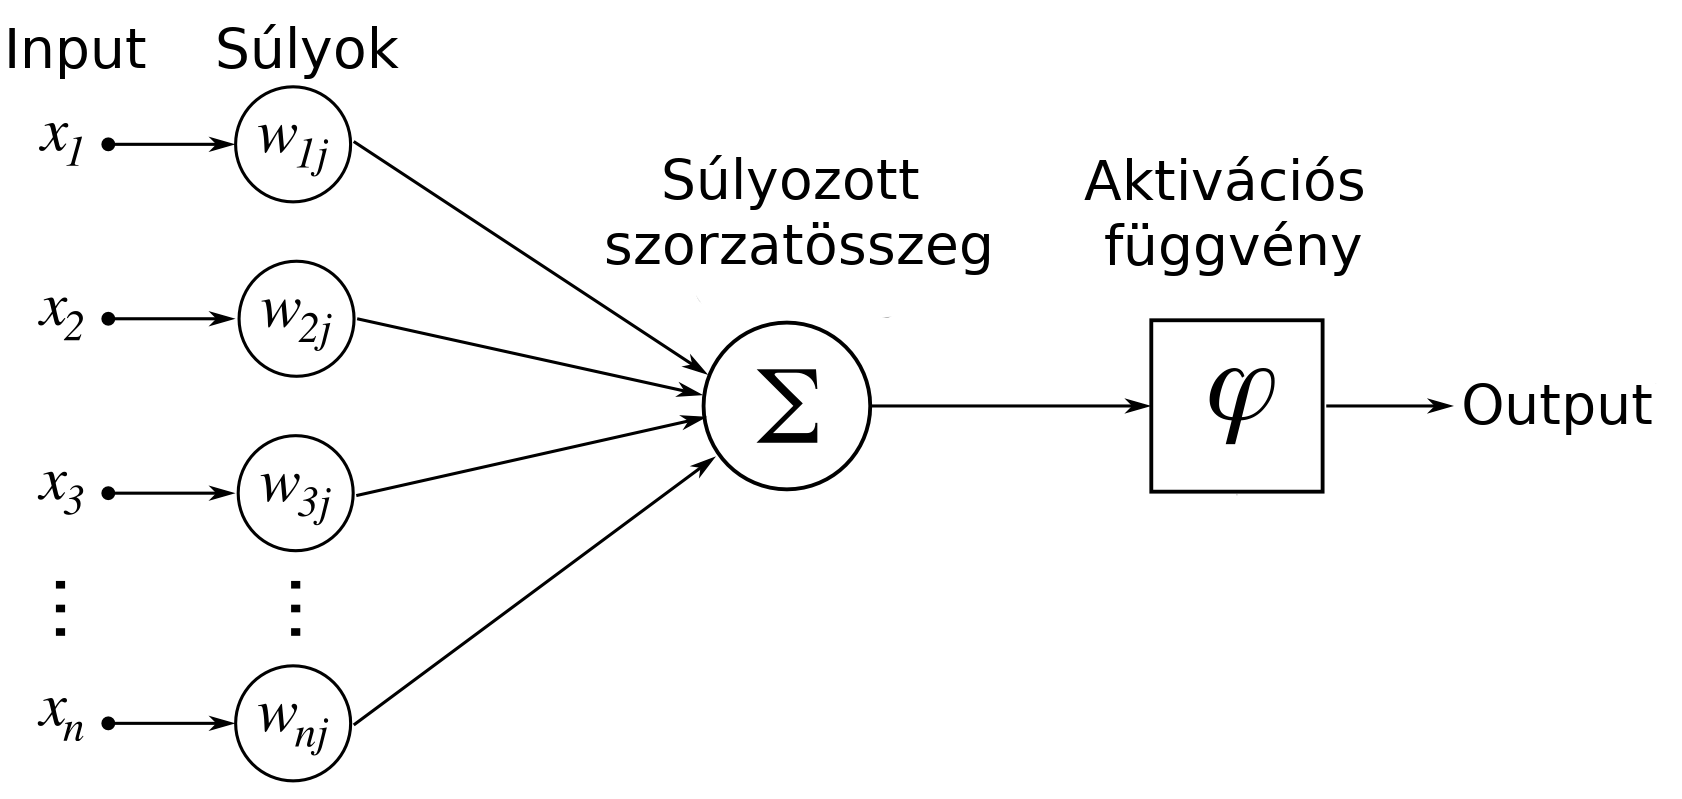
\includegraphics[width=9cm, keepaspectratio]{../../5_ql/doc/images/ql_21.png}
\end{center}
\end{column}
\end{columns}
\end{frame}

\begin{frame}{Gyakori aktivációs függvények}
\begin{columns}
\begin{column}{.5\textwidth}
A neuron által kiszámolt súlyozott szorzatösszeg egy aktivációs függvénybe kerül behelyettesítésre. \par\smallskip
A neurális hálózatok az aktivációs függvények segítségével \textbf{sajátítanak el komplex mintázatokat}. Az aktivációs függvény vezeti be a neurális hálózatokba a \textbf{nemlineáris transzformációt}, enélkül csak egy lineáris transzformáció lenne.\par\smallskip
A különböző alkalmazásokra külön aktivációs függvények használatosak.
\end{column}
\begin{column}{.5\textwidth}
\begin{center}
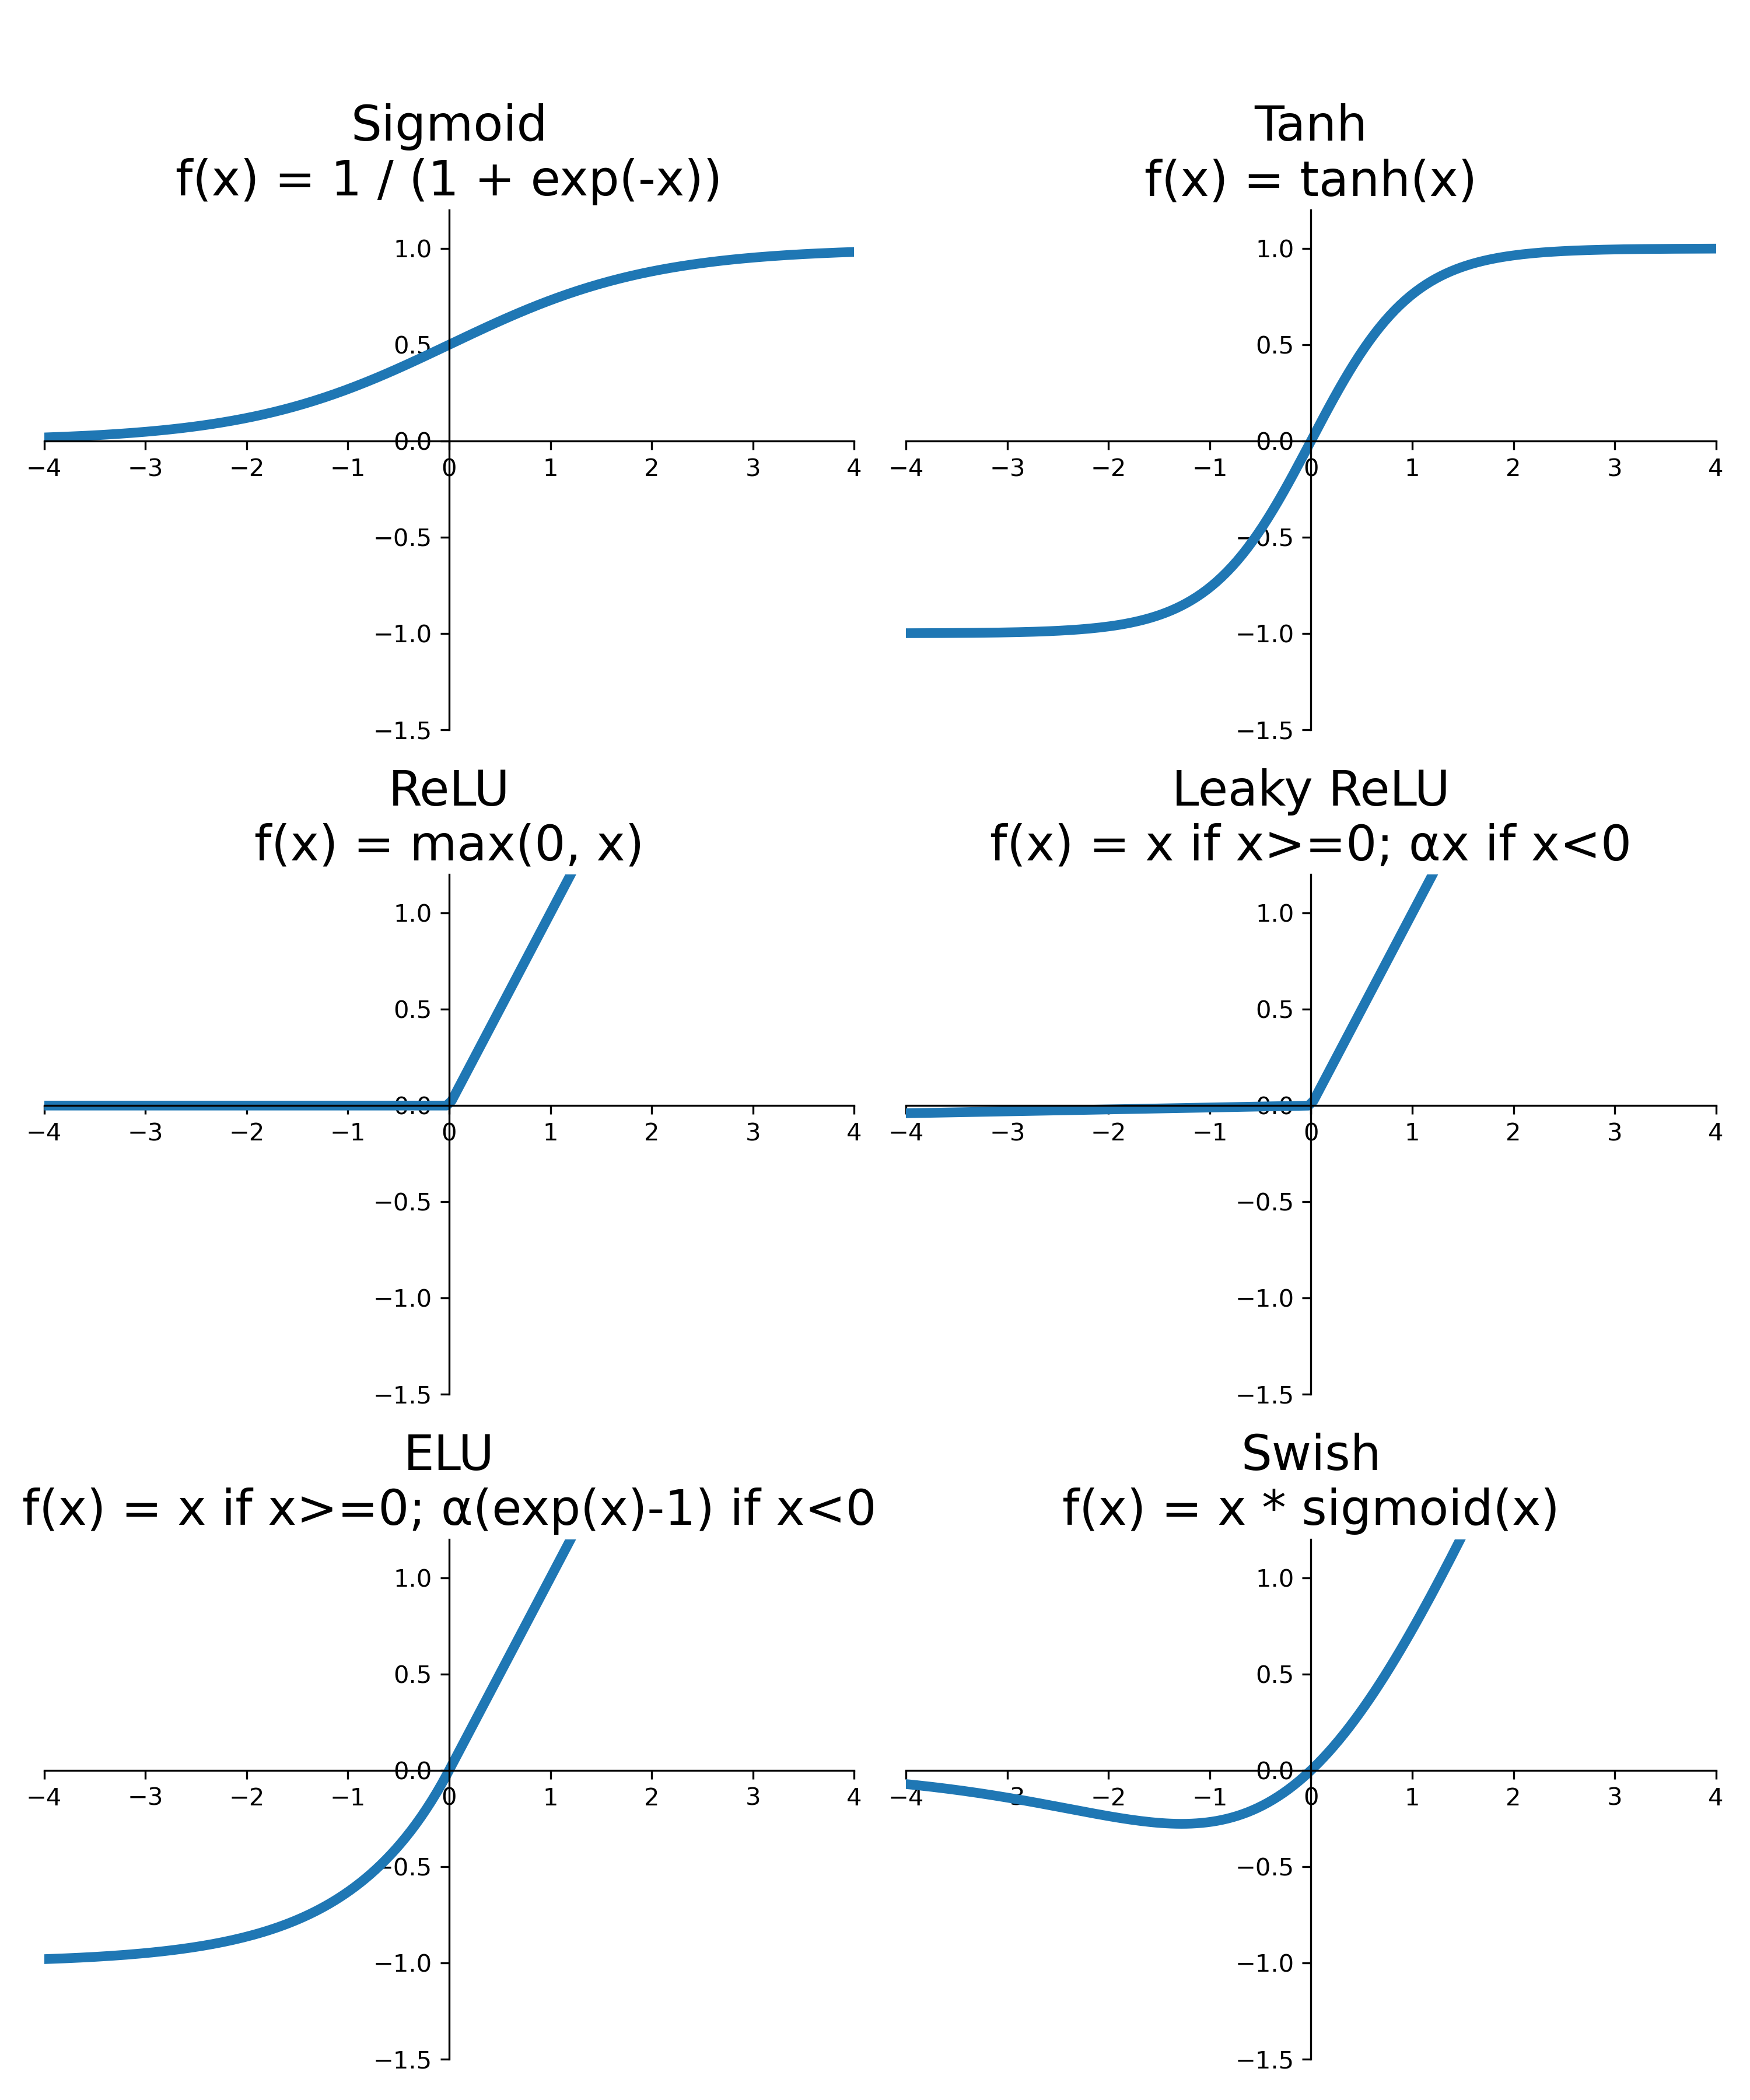
\includegraphics[height=7cm, keepaspectratio]{images/dl_2.png}
\end{center}
\end{column}
\end{columns}
\end{frame}

\begin{frame}{Többrétegű hálózatok}
\begin{columns}
\begin{column}{.5\textwidth}
Ebben az esetben a neuronok rétegekben foglalnak helyet. A kapcsolataik az előző réteg kimeneteivel állnak összeköttetésben. A legelső réteg neuronjai a bemeneti adattal állnak összeköttetésben. Minden bemeneti jellemzőhöz egy neuron tartozik.\par\smallskip
\begin{block}{Teljesen becsatolt neuronréteg kimenete}
\[
h_{W,b}(X)=\varphi(XW+b)
\]
\vspace{-0.5cm}
\begin{itemize}
	\item $X$: Input jellemzők mátrixa
	\item $W$: Kapcsolati súlyok mátrixa
	\item $b$: Torzítások vektora
	\item $\varphi$: Aktivációs függvény
\end{itemize}
\end{block}
\end{column}
\begin{column}{.5\textwidth}
\begin{center}
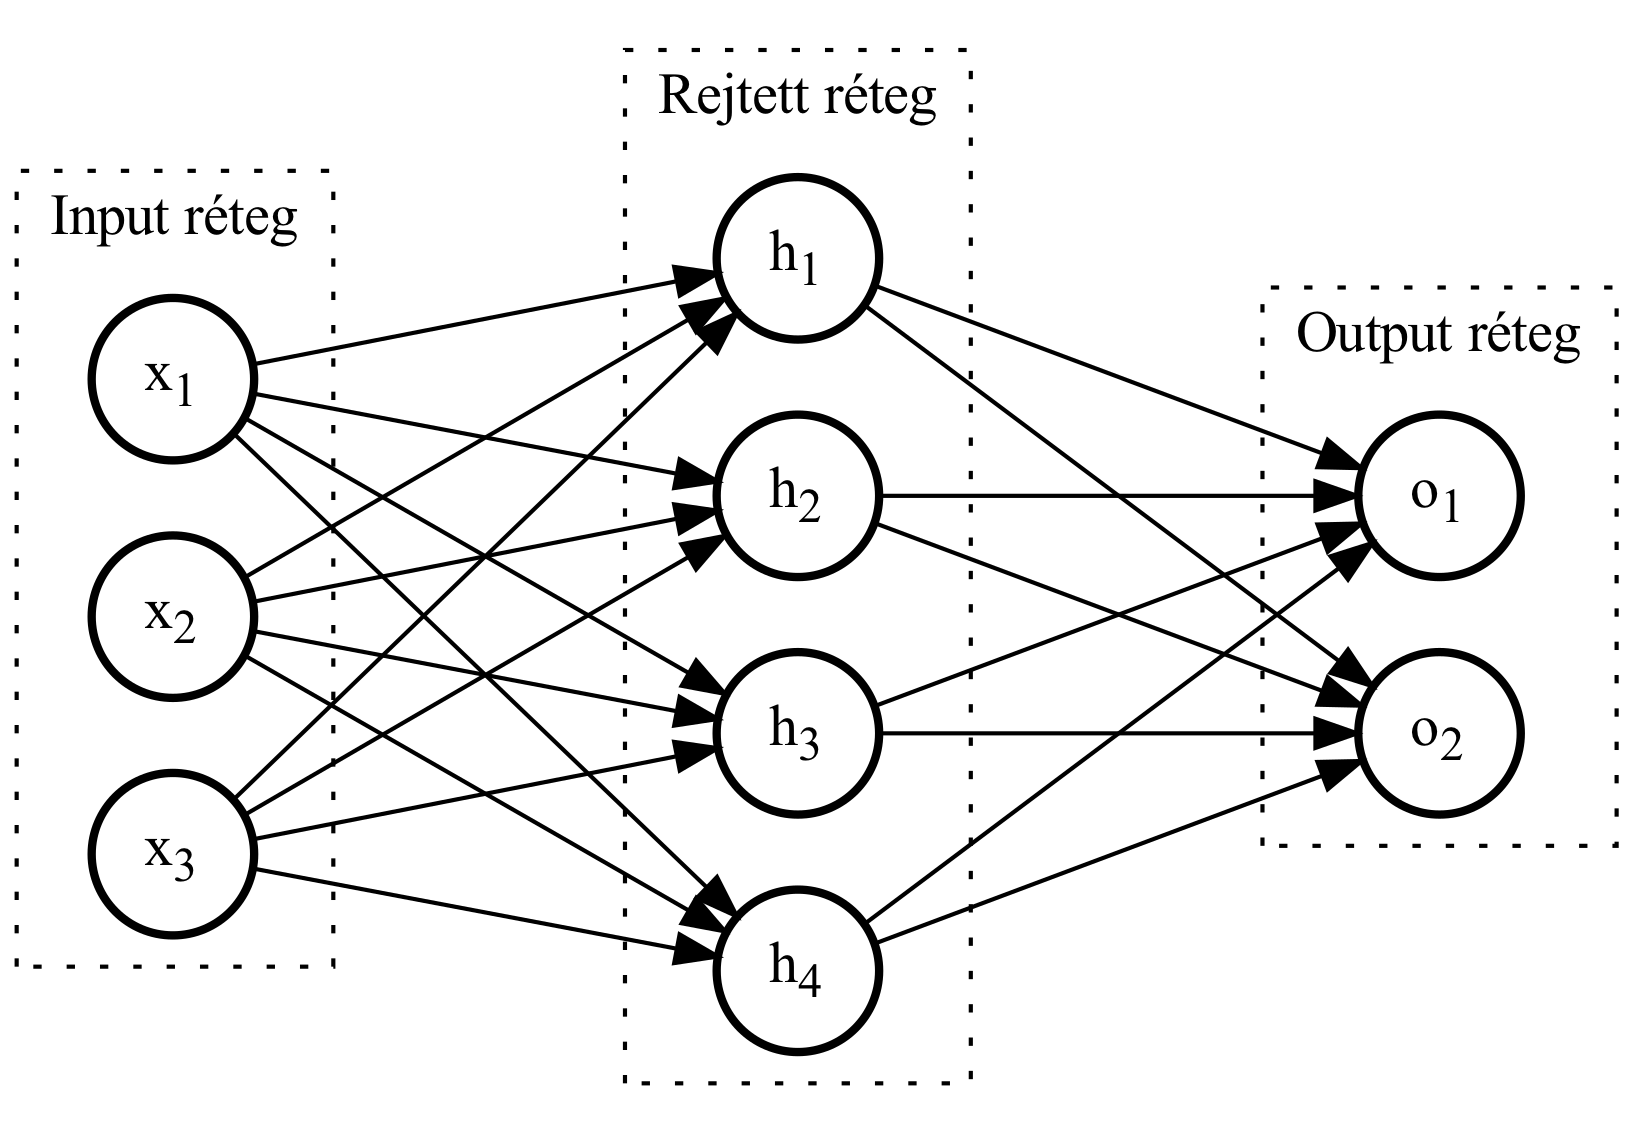
\includegraphics[width=7cm, keepaspectratio]{graphs/dl_0.png}
\end{center}
\end{column}
\end{columns}
\end{frame}

\begin{frame}{Hálózati architektúrák}
\begin{columns}
\begin{column}{.5\textwidth}
\only<1>{A regressziós problémák esetén a neurális hálónak \textbf{egyetlen output neuronja} van.\par\smallskip
A regresszió \textbf{tárgya egy folytonos} változó. Ebben az esetben a neuron output értéke a neurális hálózat predikciója a célváltozóra vonatkozóan.\par\smallskip
\textbf{Például}: hány fok lesz holnap este?\\
- 35.}
\only<2>{Az osztályozási problémák tárgya \textbf{egy diszkrét változó}, amely különálló kategóriákra osztható.\par\smallskip
Az osztályozó hálózatnak \textbf{annyi output neuronja van, ahány kategória lehetséges osztályozás esetén}. A predikció a mintaegyed adott osztályba esésének valószínűségét adja.\par\smallskip
\textbf{Például}: meleg vagy hideg lesz az idő holnap este?\\
- Hideg.}
\end{column}
\begin{column}{.5\textwidth}
\only<1>{\begin{center}
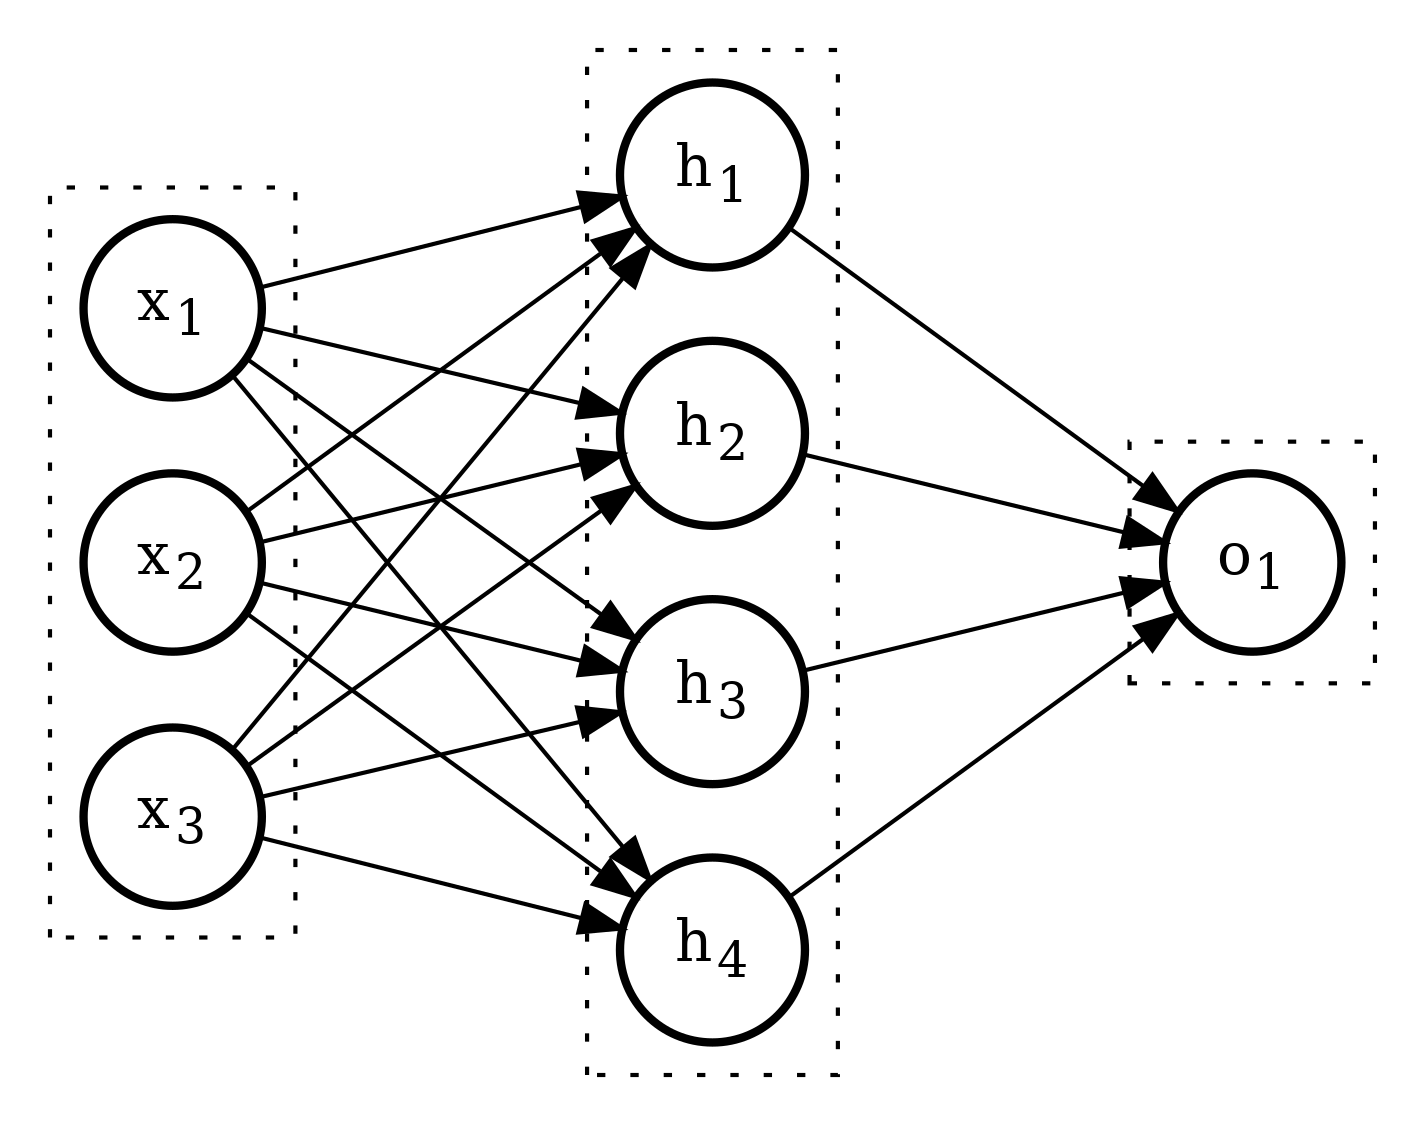
\includegraphics[width=7cm, keepaspectratio]{graphs/dl_2.png}
\end{center}}
\only<2>{\begin{center}
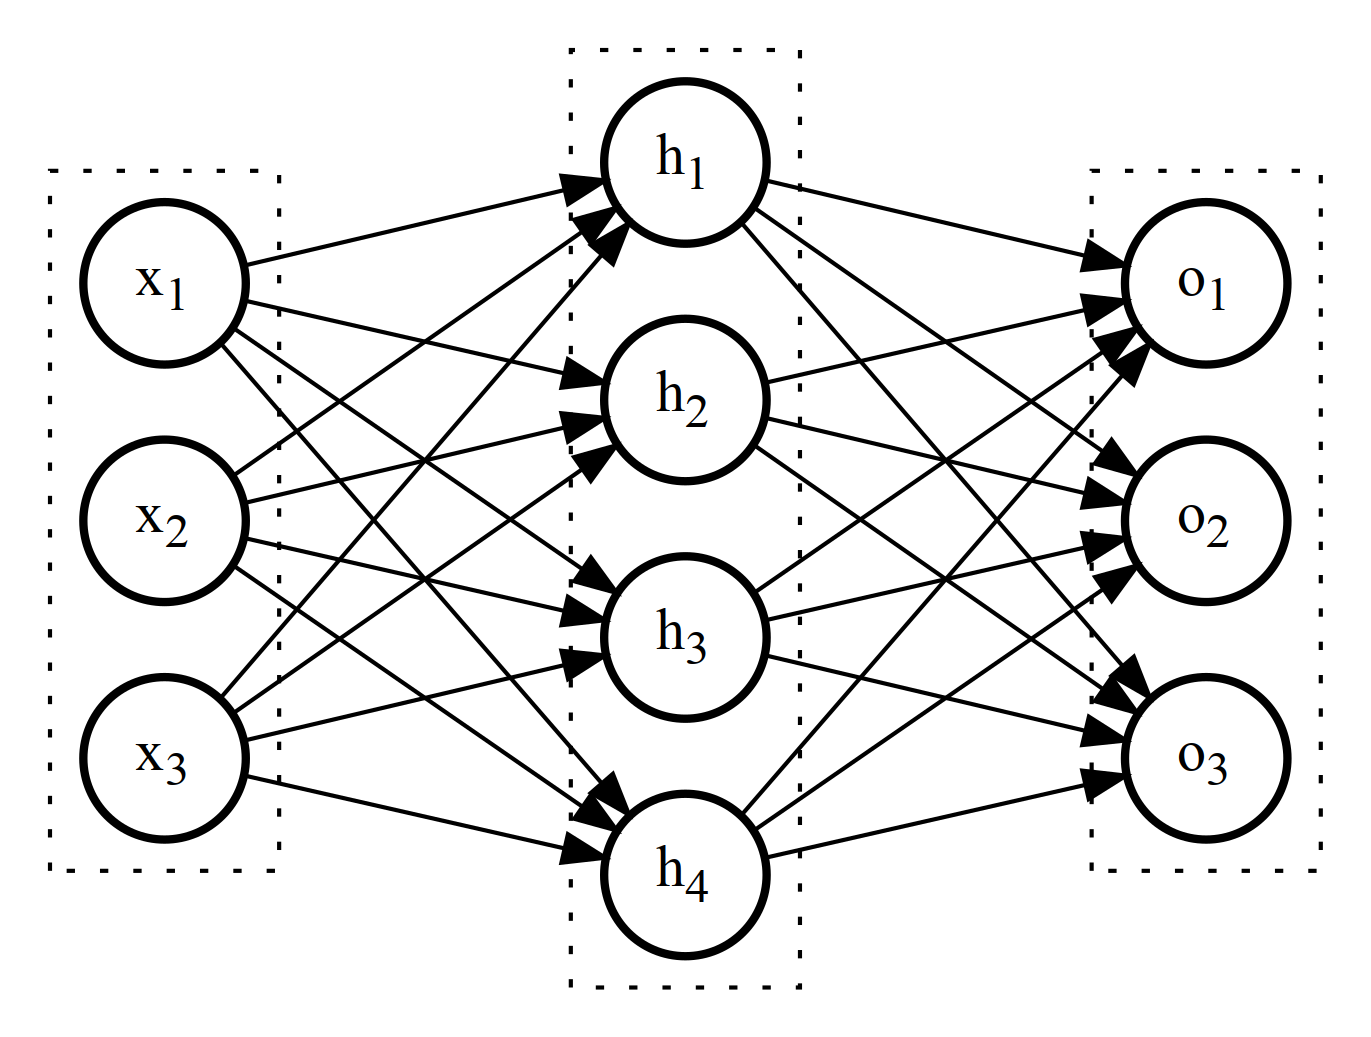
\includegraphics[width=7cm, keepaspectratio]{graphs/dl_1.png}
\end{center}}
\end{column}
\end{columns}
\end{frame}

\section{Tanítás}

\begin{frame}
\tableofcontents[currentsection]
\end{frame}

\begin{frame}{Hiba-visszaáramoltató algoritmus neurális hálózat súlyok tanítására}
\begin{enumerate}
	\item \textbf{Inicializáció}: súlyok és torzítások kezdőértékeinek véletlenszerű megadása
	\item \textbf{Előreáramoltatás}: rétegek output értékének kiszámítása: 
	\begin{itemize}
		\item Rejtett réteg: $h_h = \varphi(W_h \cdot x + b_h)$
		\item Output réteg: $h_o = \varphi(W_o \cdot h_h + b_o)$
	\end{itemize}
	\item \textbf{Költség kiszámítása}: regresszió esetén pl.: $MSE = \sum \left( h_o - y \right)$
	\item \textbf{Visszaáramoltatás}: 
	\begin{itemize}
		\item Rejtett réteg hibája: $\delta_h=(W_o \cdot \delta_o) \odot \varphi(z_h)$
		\item Output réteg hibája: $\delta_o=(h_o - y) \odot \varphi(z_o)$
	\end{itemize}
	\item \textbf{Gradiens ereszkedés} a súlyokon és torzításokon:
	\begin{itemize}
		\item Rejtett réteg: $W_h \leftarrow W_h - \alpha \cdot \delta_h \cdot x^\top$
		\item Rejtett réteg: $b_h \leftarrow b_h - \alpha \cdot \delta_h$	
		\item Output réteg: $W_o \leftarrow W_o - \alpha \cdot \delta_o \cdot h_o^\top$
		\item Output réteg: $b_o \leftarrow b_o - \alpha \cdot \delta_o$

	\end{itemize}
	\item \textbf{Ismétlés} a meghatározott lépésszámig
\end{enumerate}
\end{frame}

\begin{frame}{Transzfertanulás}
\begin{columns}
\begin{column}{.5\textwidth}
Neurális hálózatok esetén lehetséges más neurális hálózatok \textbf{előretanított súlyainak felhasználása}. Ebben az esetben adott rétegek kimaradnak a tanításból.\par\smallskip
Jellemzően az alsó rétegek lesznek rögzítettek, és a felső rétegek pedig tanítottak. Ez lehetőséget ad a hálózatnak \textbf{új mintázatokat megismerni hasonló feladatok} esetén.
\end{column}
\begin{column}{.5\textwidth}
\begin{center}
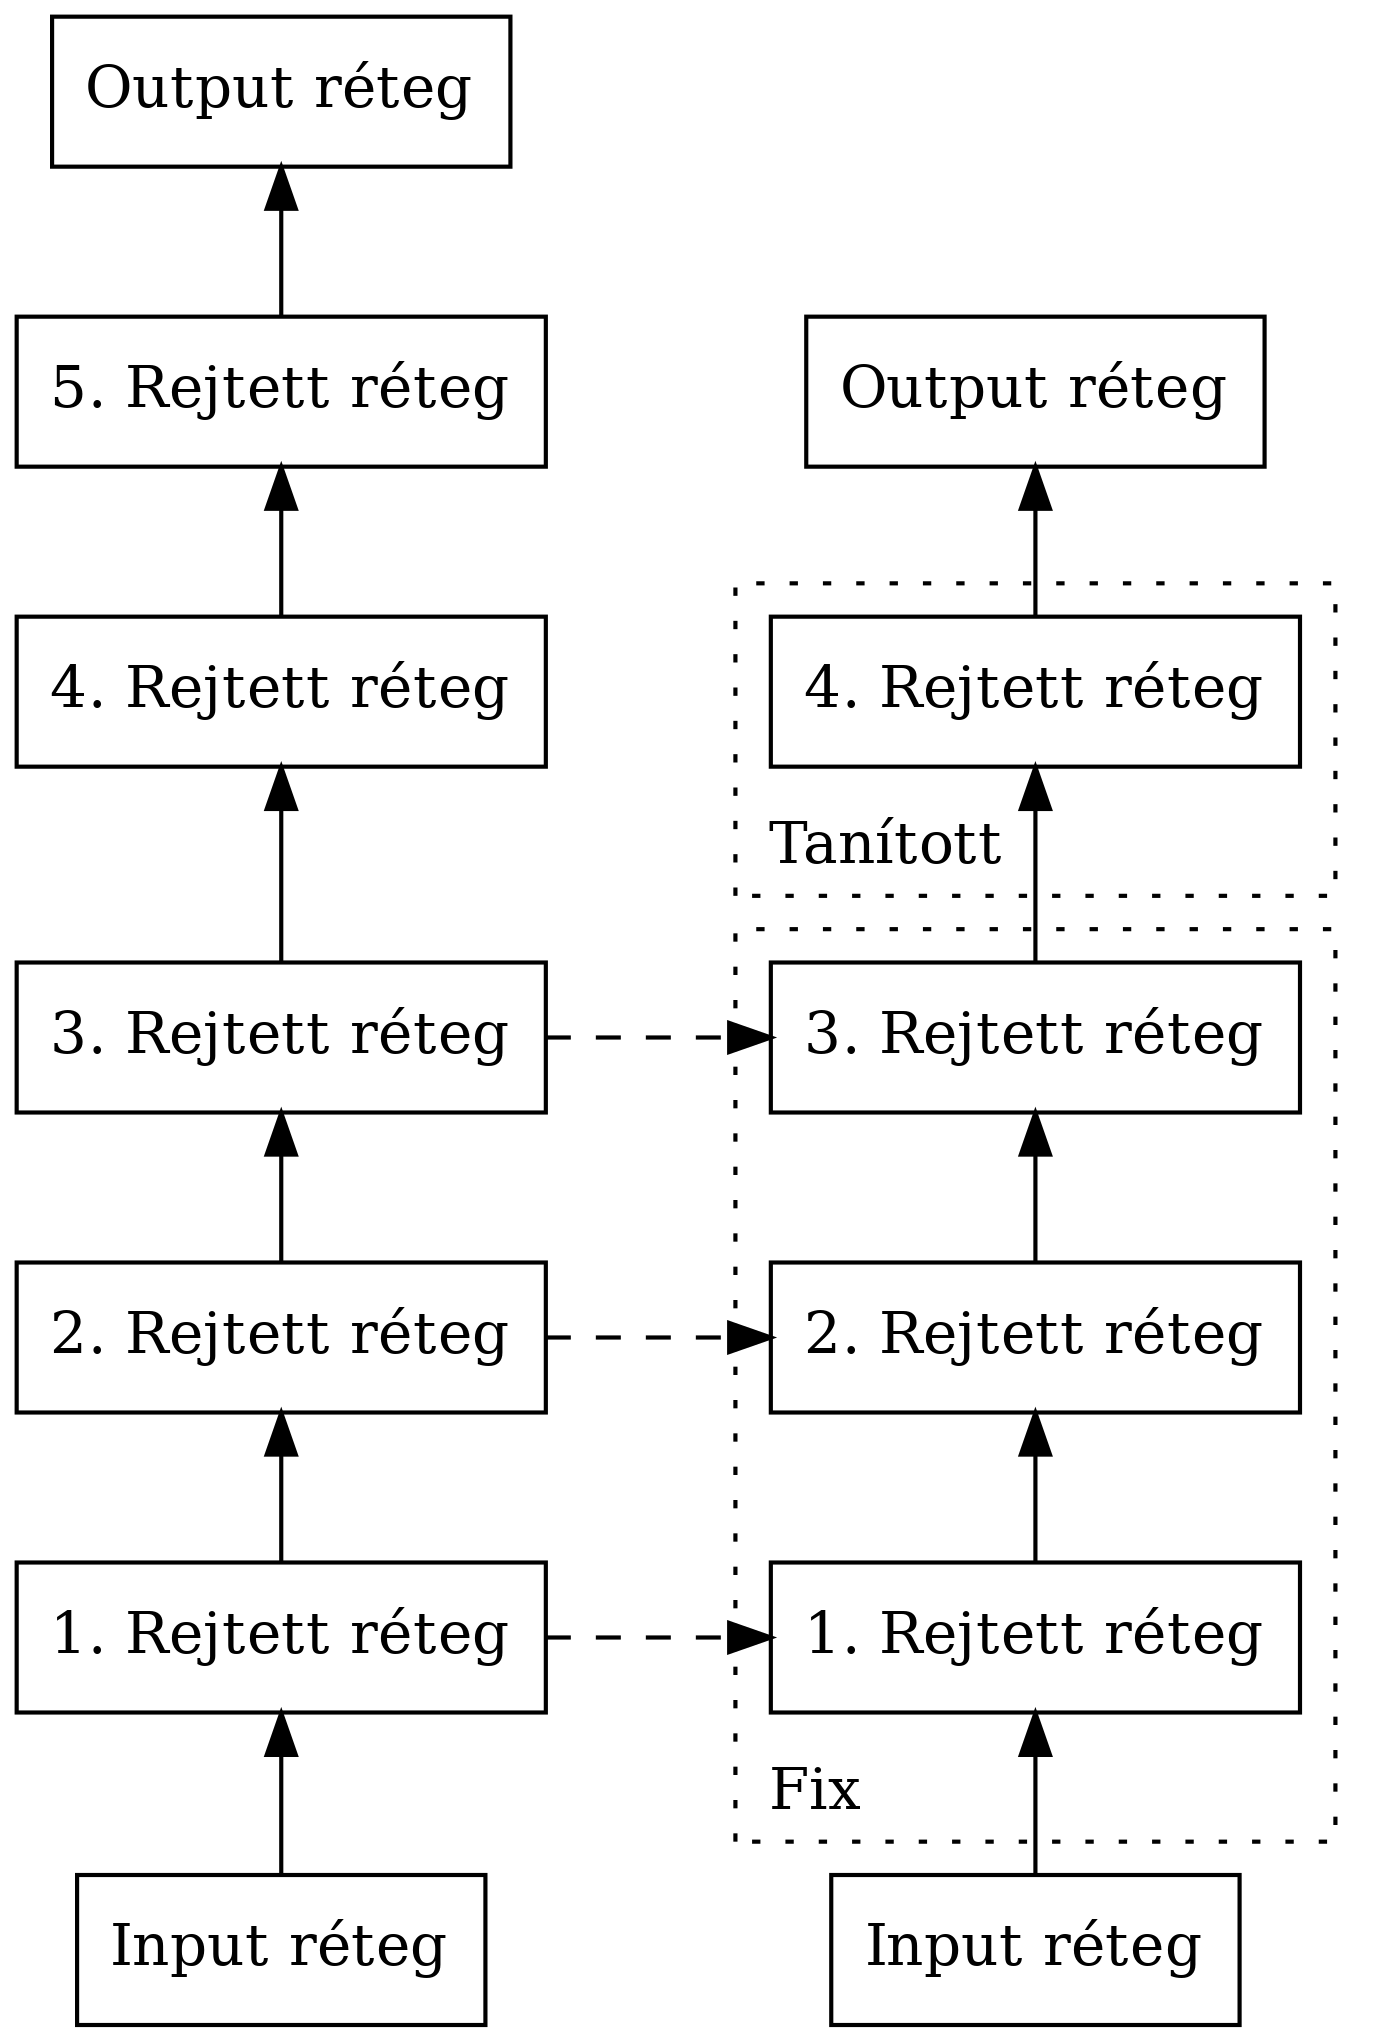
\includegraphics[height=7cm, keepaspectratio]{graphs/dl_3.png}
\end{center}
\end{column}
\end{columns}
\end{frame}

\begin{frame}{Optimalizációs algoritmusok}
\begin{columns}
\begin{column}{.5\textwidth}
A matematikában az optimalizációs algoritmusok melyeknek célja megtalálni a legjobb megoldást egy olyan problémára, ahol valamilyen korlátozásokkal kell \textbf{egy célfüggvényt minimalizálni}.\par\smallskip
Mivel a neurális hálók által reprezentált nemlineáris függvények minimum helyei nem számíthatók ki zárt formájú függvénnyel, az optimalizáló algoritmusok iteratívak. 
\end{column}
\begin{column}{.5\textwidth}
\begin{center}
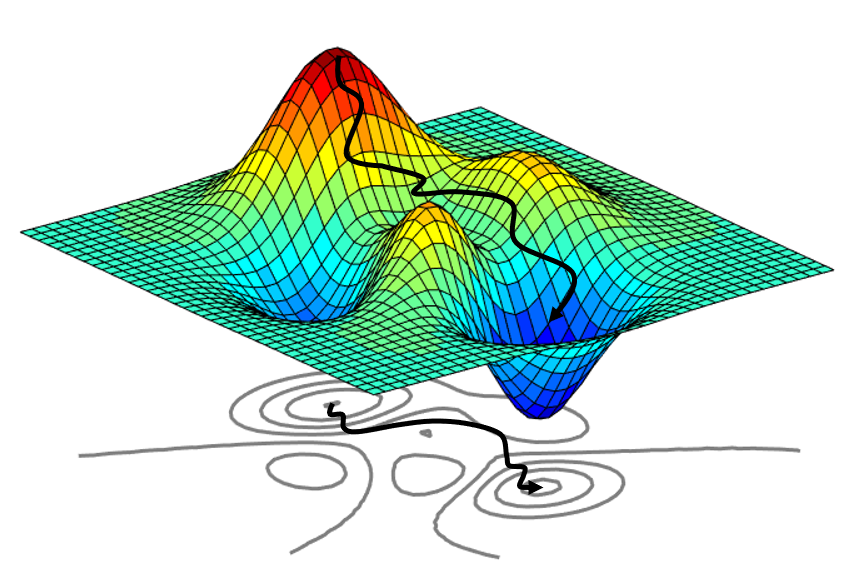
\includegraphics[height=7cm, width=7cm, keepaspectratio]{images/dl_8.png}
\end{center}
\end{column}
\end{columns}
\end{frame}

\begin{frame}{Gradiens ereszkedés}
\begin{columns}
\begin{column}{.5\textwidth}
% ITT TARTOK
\end{column}
\begin{column}{.5\textwidth}

\end{column}
\end{columns}
\end{frame}

\section{Konvolúciós hálózatok}

\begin{frame}
\tableofcontents[currentsection]
\end{frame}

\begin{frame}{A konvolúció művelete}
\begin{columns}
\begin{column}{.6\textwidth}
A konvolúció egy matematikai művelet, ami két függvényt kombinál egy harmadikká. Egy \textbf{jelfüggvényt} valamilyen \textbf{magfüggvénnyel} vegyít egy outputtá, ami megadja, hogy \textbf{a mag mennyiben befolyásolja a jelet}. 
\begin{block}{Konvolúció (2D, diszkrét)}
A diszkrét konvolúció két 2D tömbön értelmezett, és jellemzők kivonatolására, szűrők alkalmazására használatos. Konvolúció $f$ jelen és $g$ magon, $i,j$ képkoordinátákra:
\[
(f \textasteriskcentered g)[i, j] = \sum_{m=-\infty}^\infty \sum_{n=-\infty}^\infty g[i-m, j-n]f[m,n]
\]
\end{block}
\end{column}
\begin{column}{.4\textwidth}
\begin{center}
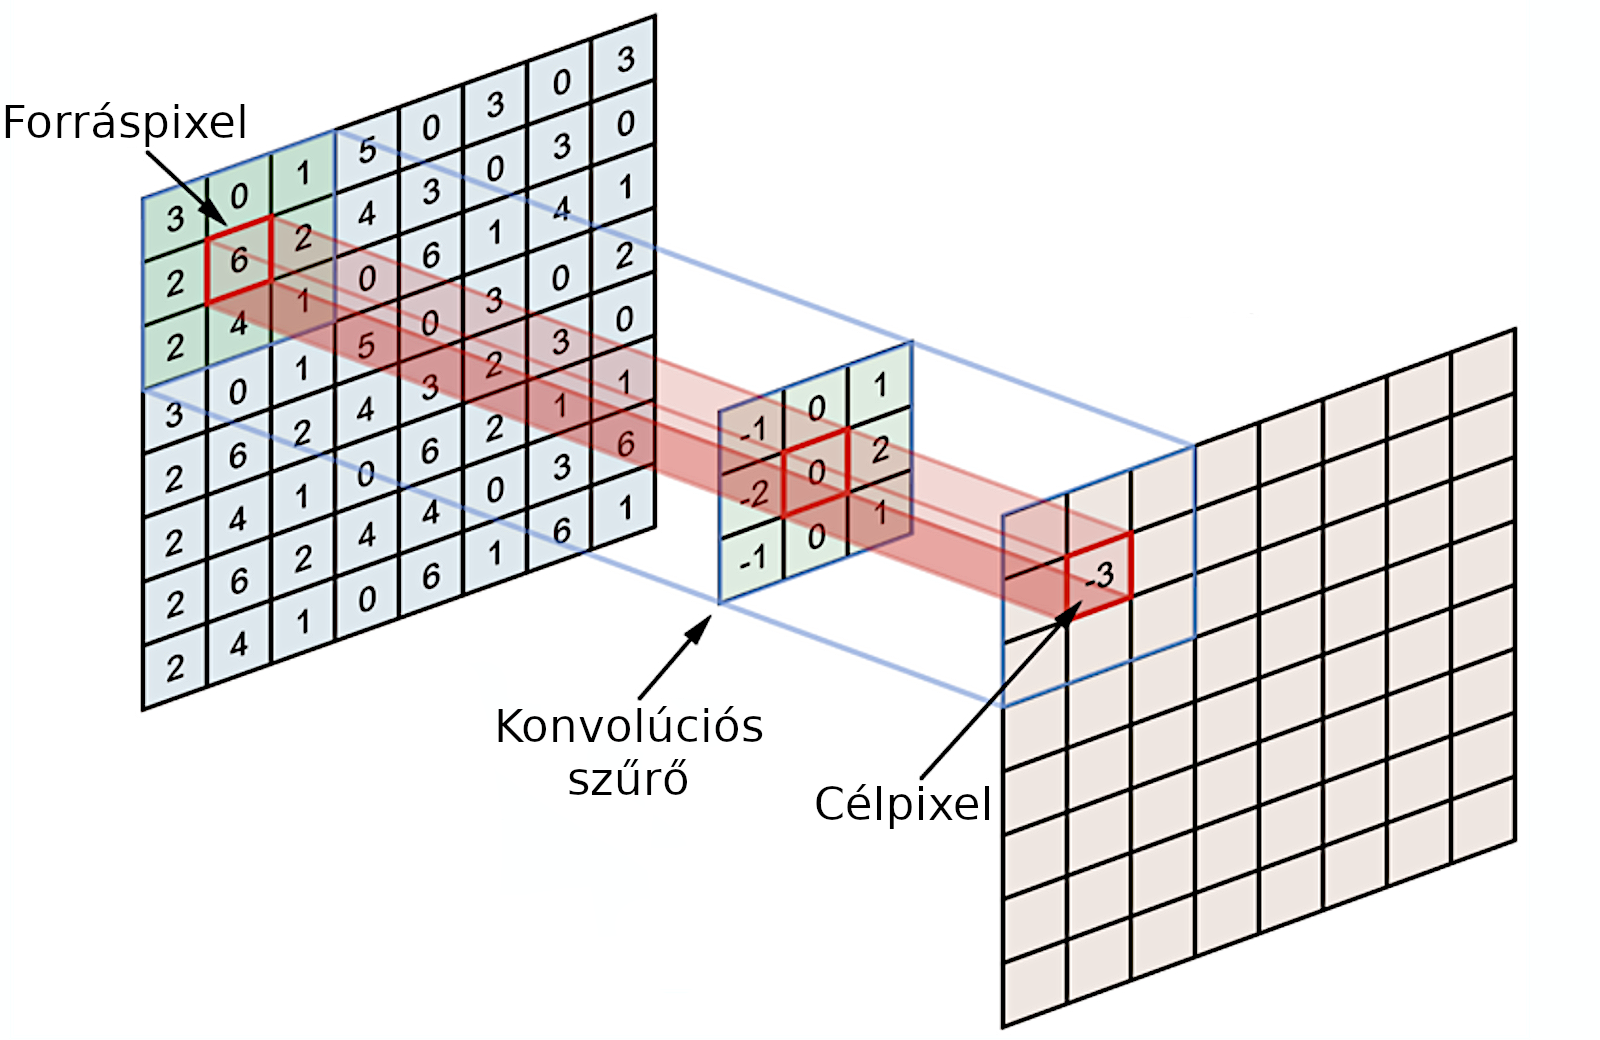
\includegraphics[height=6cm, width=6cm, keepaspectratio]{images/dl_3.png}
\end{center}
$(-1 \cdot 3) + (0 \cdot 0) + (1 \cdot 1) +$\\
$(-2 \cdot 2) + (0 \cdot 6) + (2 \cdot 2) +$\\
$(-1 \cdot 2) + (0 \cdot 4) + (1 \cdot 1) = -3$\\
\end{column}
\end{columns}
\end{frame}

\begin{frame}{A konvolúciós réteg}
\begin{columns}
\begin{column}{.5\textwidth}
A neurális hálózatok konvolúciós rétegeiben a \textbf{tanítható súlyok az egyes forráspixelekhez tartozó konvolúciós szűrőkben elhelyezkedő értékek}. Ez minden forráspixelhez egy egyedi szűrőt jelent, de lehetséges tetszőleges számú szűrő is.\par\smallskip
A konvolúciós magfüggvények szűrőként is alkalmazhatók. Például a képen egy élkereső szűrő látható, ami az outputra az input képen található élek másolódnak át.\par\smallskip  
\end{column}
\begin{column}{.5\textwidth}
\begin{center}
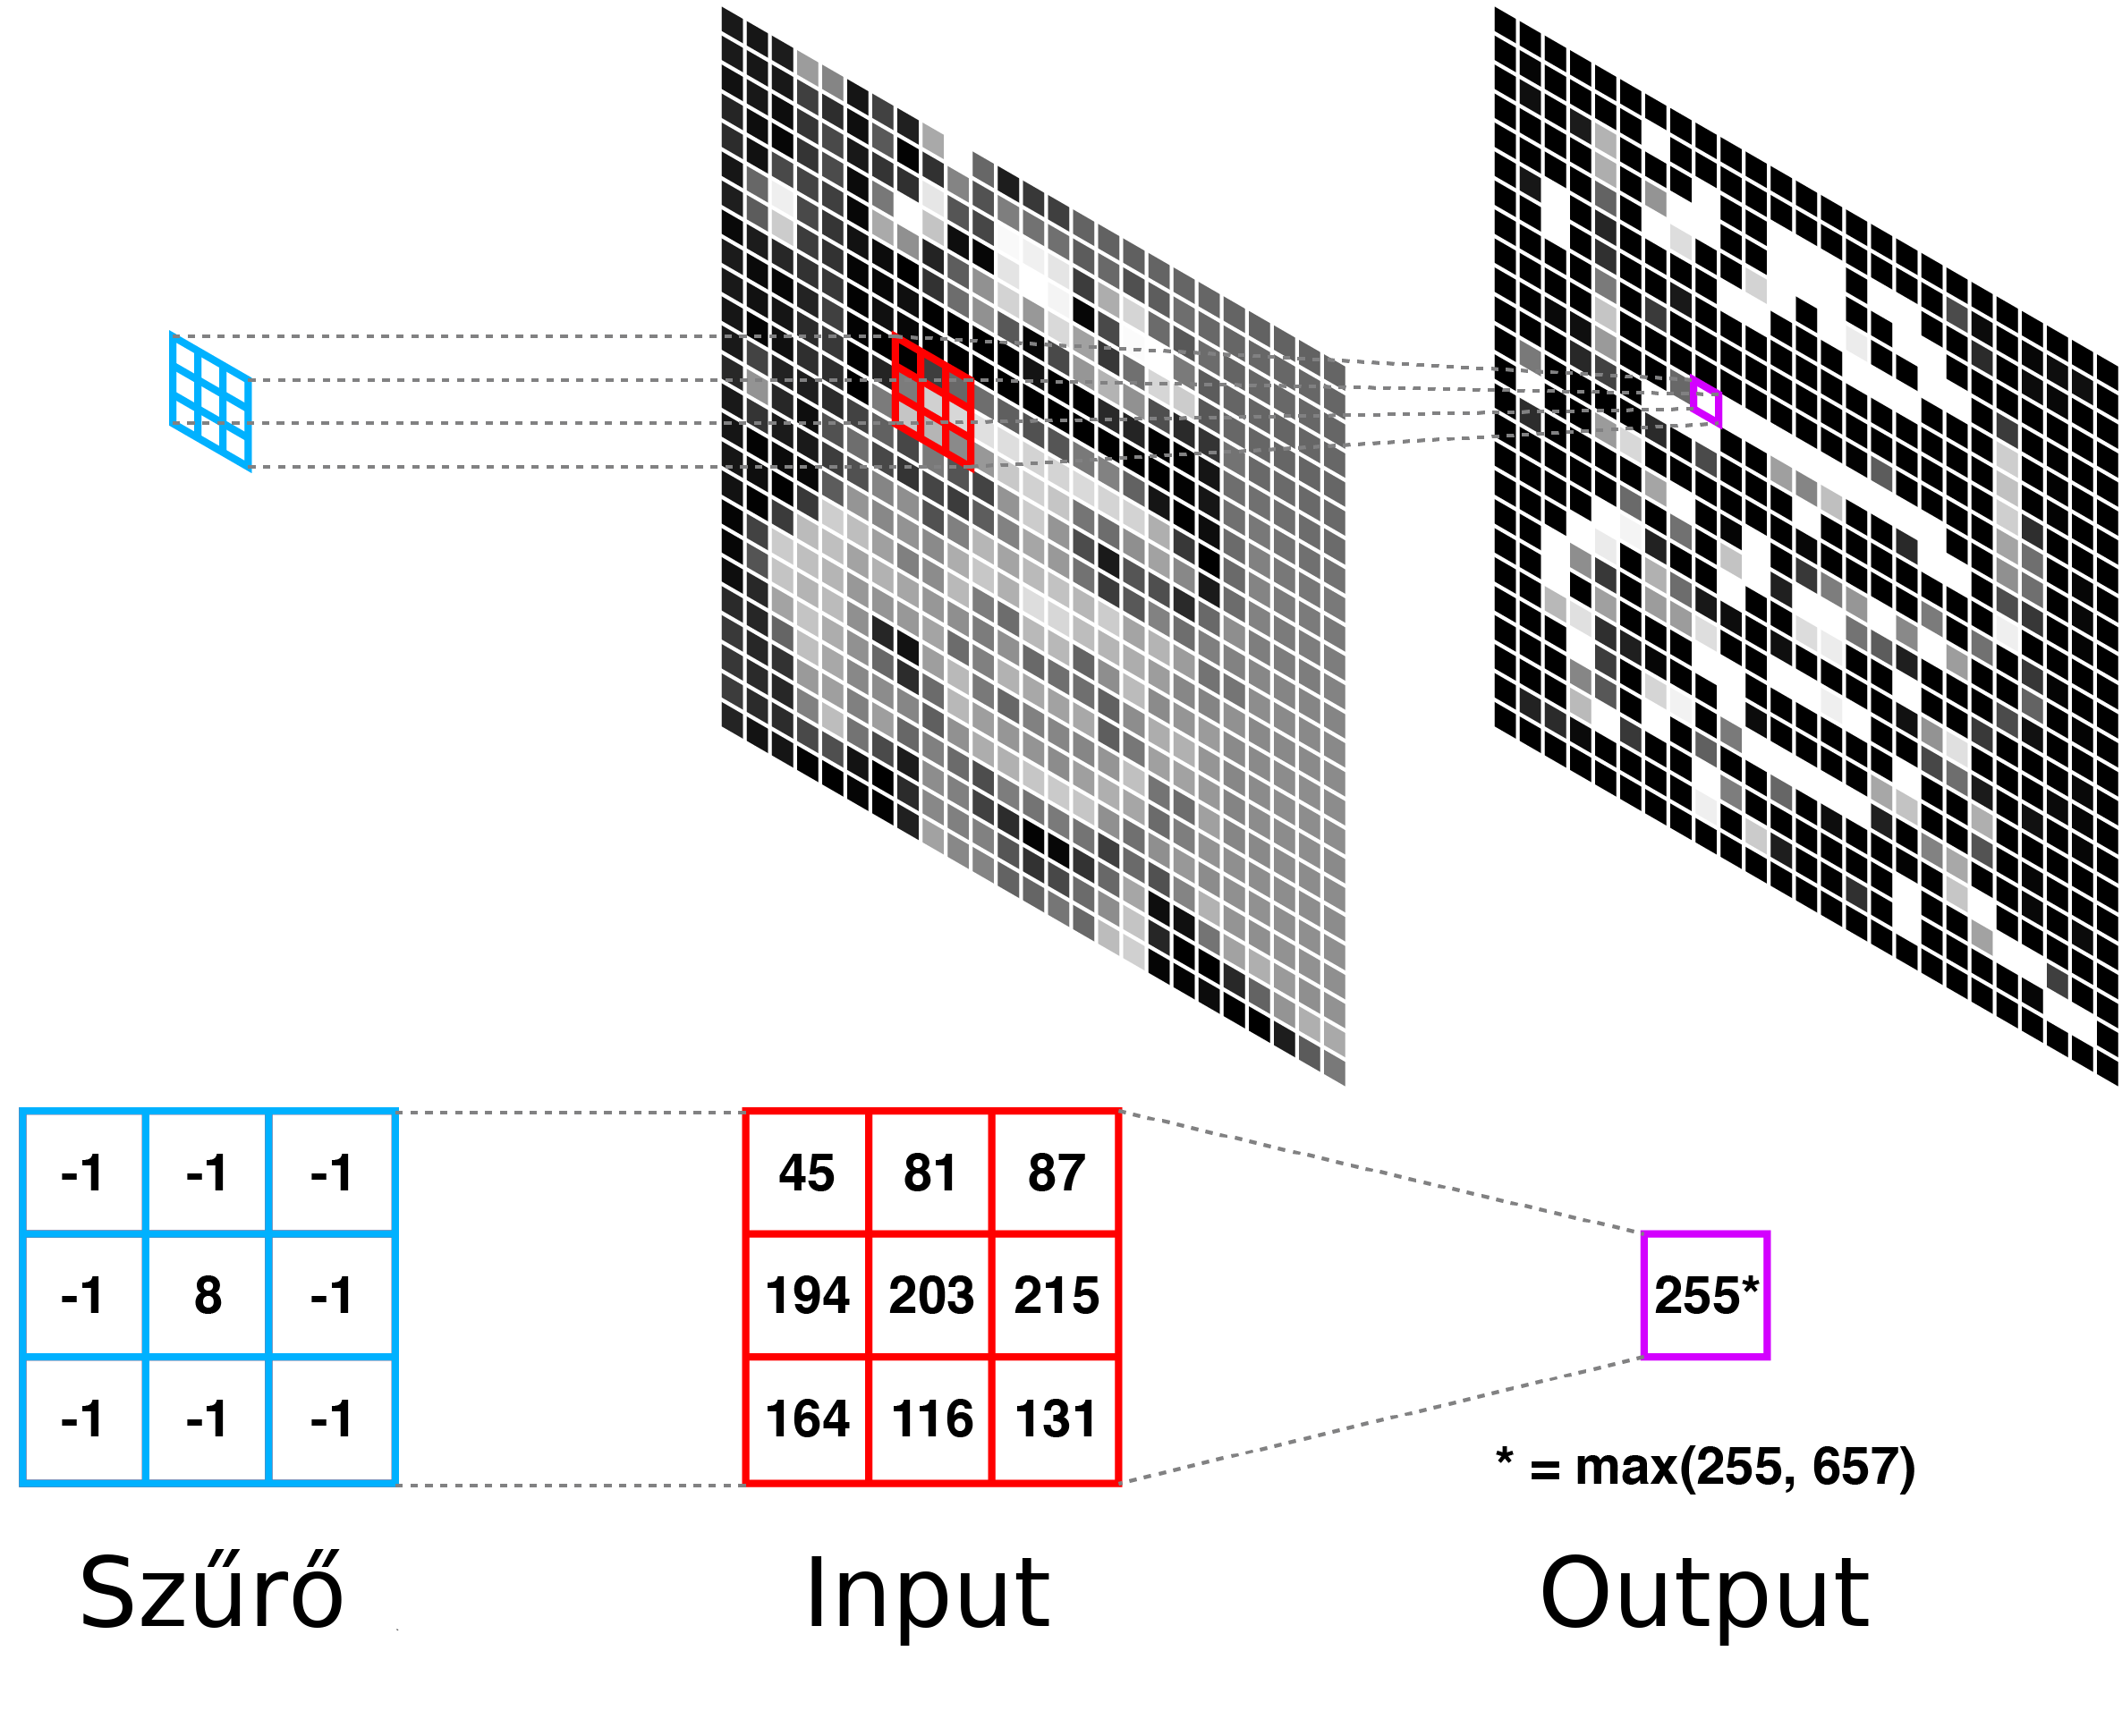
\includegraphics[height=7cm, width=7cm, keepaspectratio]{images/dl_4.png}
\end{center}
\end{column}
\end{columns}
\end{frame}

\begin{frame}{Konvolúció több dimenzióban}
\begin{columns}
\begin{column}{.5\textwidth}
A konvolúció általánosítható több dimenzióra is. A gyakorlatban 3D konvolúció megy végbe a neurális hálózatokban, \textbf{hiszen a színes képek 3D mátrixokban tárolódnak el}, ahol az egyes dimenziók a \emph{magasság, hosszúság és csatorna}. A csatorna három elemű és az R,G,B értékeket kódolja.\par\smallskip
A konvolúció tetszőleges dimenzióra általánosítható művelet.
\end{column}
\begin{column}{.5\textwidth}
\begin{center}
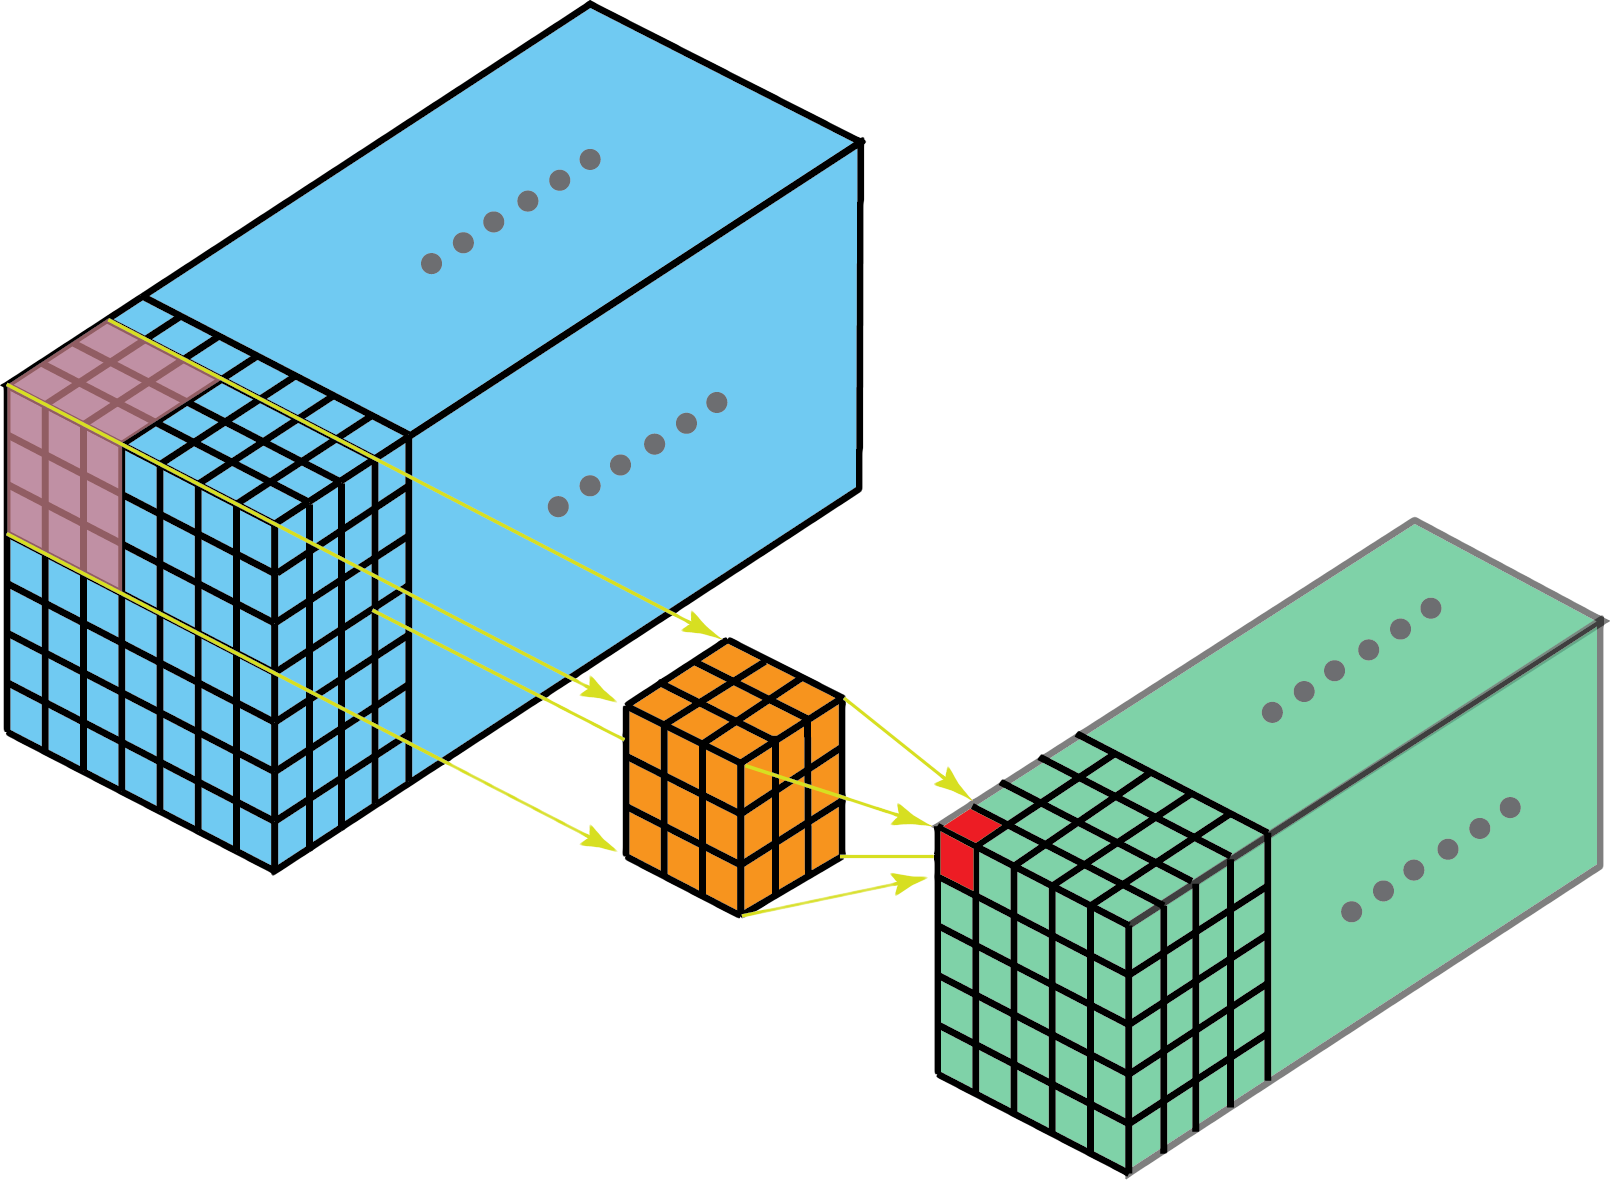
\includegraphics[height=7cm, width=7cm, keepaspectratio]{images/dl_5.png}
\end{center}
\end{column}
\end{columns}
\end{frame}

\begin{frame}{Pooling réteg}
\begin{columns}
\begin{column}{.5\textwidth}
A pooling vagy lazítás egy almintázási művelet, ami csökkenti a \textbf{bemenet térbeli dimenzióit}, miközben a fontos információt megtartja. A konvolúciós hálózatokban gyakran használatos a számítási igény csökkentésére, túltanulás elkerülésére és a hálózat segítésére abban, hogy fontos mintázatokat tanuljon meg.\par\smallskip
\begin{block}{Pooling neuron}
A vele kapcsolatban álló \textbf{neuronok output értékeit aggregálja valamilyen függvény szerint}. Leggyakrabban ez az \textbf{átlagolás} vagy a \textbf{maximum} kiválasztás.
\end{block}
\end{column}
\begin{column}{.5\textwidth}
\begin{center}
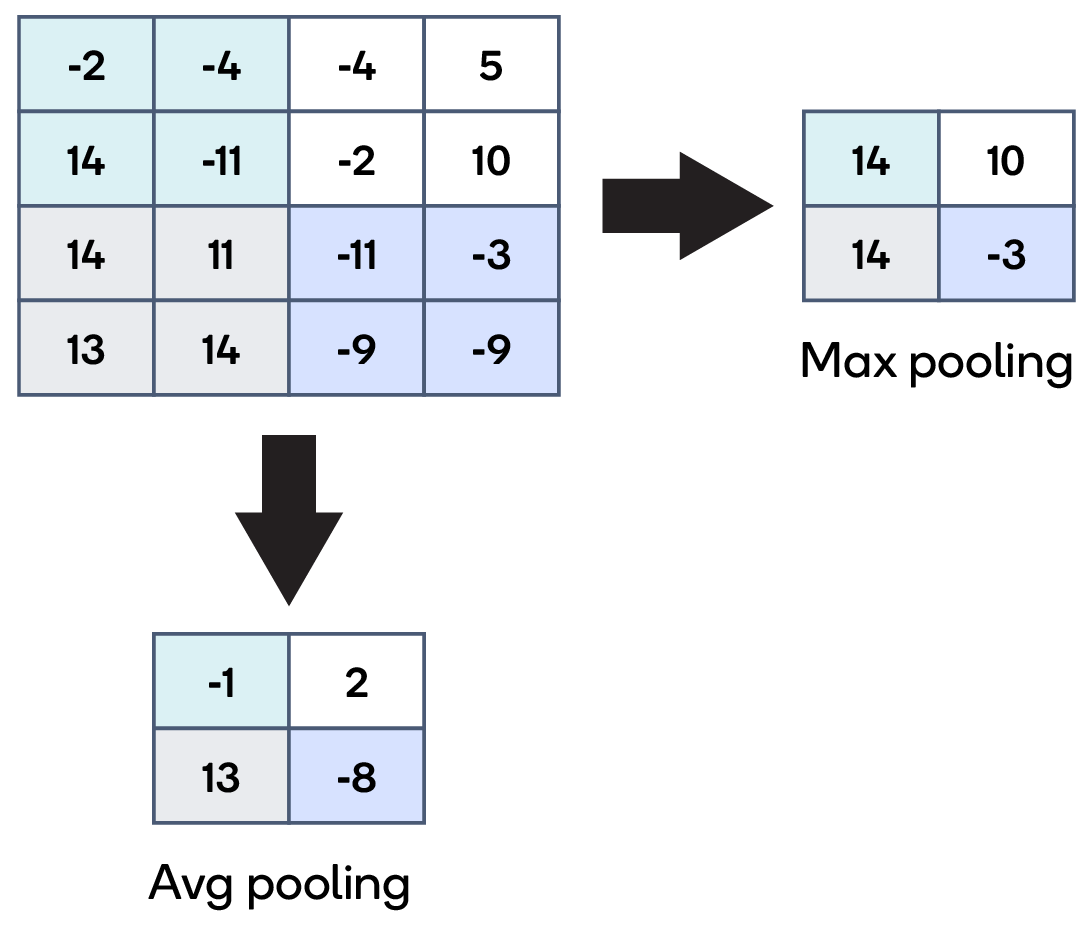
\includegraphics[height=5cm, width=7cm, keepaspectratio]{images/dl_6.png}
\end{center}
$\frac{1}{4}(-2 -4 +14 -11)=-1$\par\smallskip
$max\{-2, -4, 14, -11\}=14$
\end{column}
\end{columns}
\end{frame}

\begin{frame}{Teljes konvolúciós architektúra}
\begin{center}
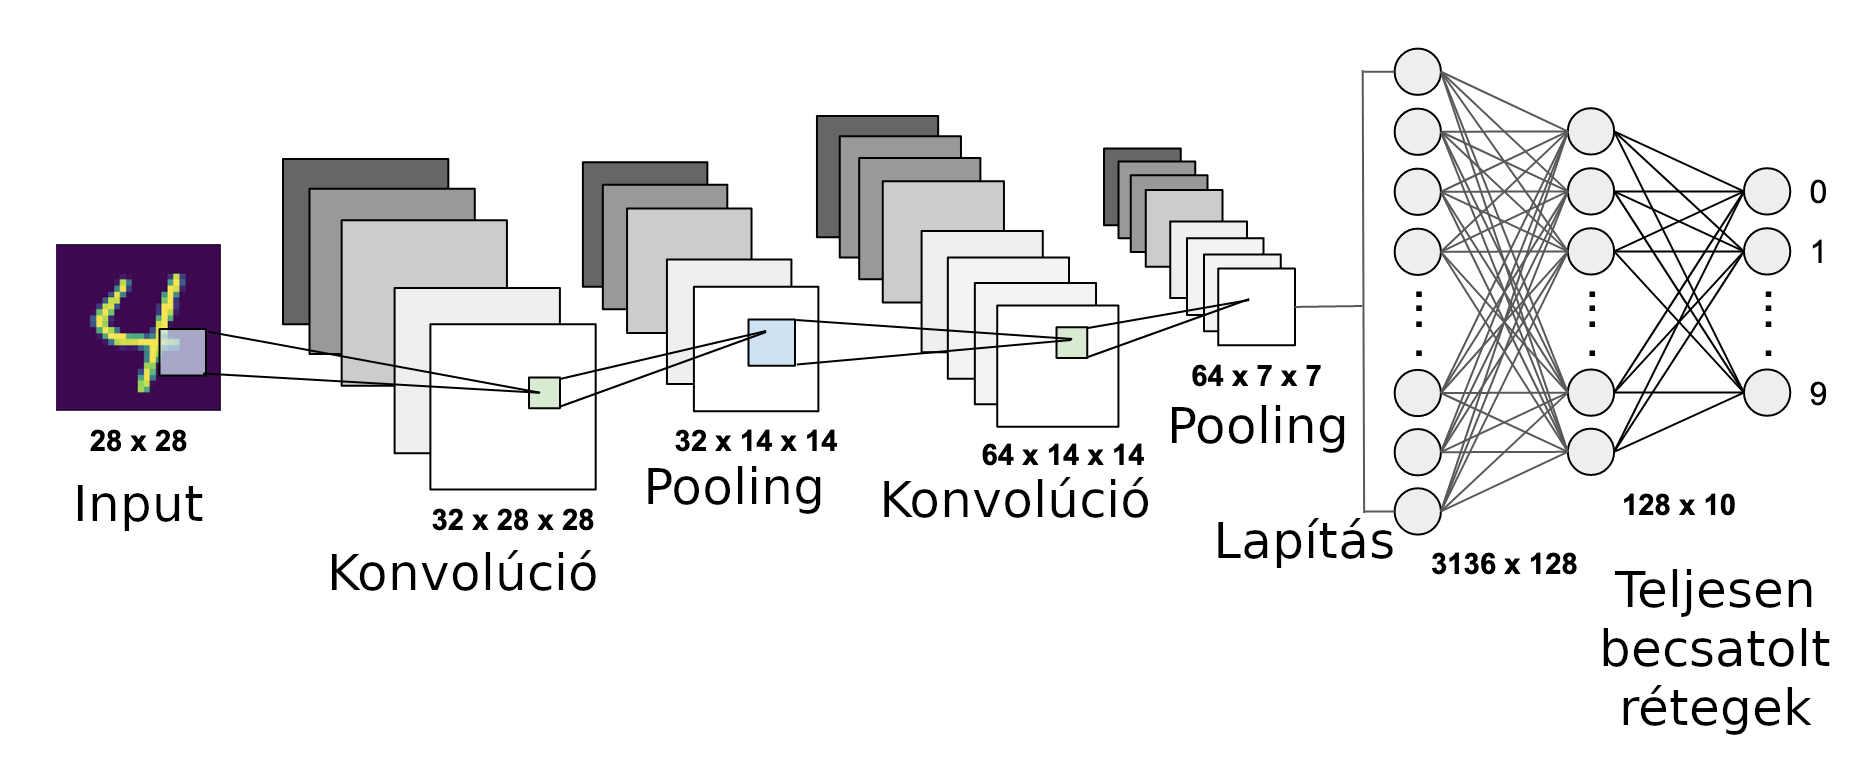
\includegraphics[height=7cm, width=14cm, keepaspectratio]{images/dl_7.png}
\end{center}
\end{frame}

\section{Önkódoló architektúrák}

\begin{frame}
\tableofcontents[currentsection]
\end{frame}


\end{document}










